\chapter{Love the Candidate but Hate his Party: The Asymmetric Effects of Reelection Incentives on Partisan and Personal Incumbency Returns in Mexico}
\section{Introduction}

Over the past decades, an important theoretical and empirical literature has shown that incumbents may enjoy an electoral advantage \citep{ashworth_2012, cox_morgensten_1993, cox_katz_1996, ansolabehere_snyder_2000, ashworth_bdm_2008, ashworth_etal_2019} or suffer from an electoral disadvantage in the next election \citep{klasnja_2015, klasnja_titiunik_2017}. However, whether positive or negative, the electoral returns from incumbency mask the returns associated to parties and those exclusively of candidates. Disentangling both measures is important to understand citizens valuation of the electoral system and the existent electoral accountability \citep{mayhew_1974, fowler_hall_2014}. For instance, a partisan incumbency advantage might imply that voters believe parties control candidates behaviors, and thus would allow parties to hold a credible threat against renegade candidates. %The implications for a personal advantage are different, however: a personal advantage makes candidates vital for parties electoral success, leading the latter to allow more leeway to the former since retiring or switching parties may hurt parties electoral success. 
However, the implications of a personal incumbency advantage are different from the partisan one. A personal incumbency advantage makes retiring politicians support of new candidates vital for their electoral success, and stepping down or switching parties may hurt their parties in the next election. In this case, parties may allow more leeway to deviate from the party line to their members.\footnote{Likewise, a partisan incumbency disadvantage may imply citizens like partisan balance across time and may create incentives for candidates to differentiate themselves from their parties \citep{klasnja_titiunik_2017}. Contrastingly, a negative personal advantage may lead parties to differentiate themselves from candidates and stop their electoral support or remove the nomination in the next election.} Moreover, if a personal (partisan) effect exists and the partisan (personal) one is negligible it implies voters attribute actions in office to candidates (parties) and not their parties (candidates) or that a party (personal) dealignment might be taking place \citep{cox_katz_1996}.   
   
However, uncovering the partisan and personal incumbency advantage has proved methodologically challenging: every time a candidate is an incumbent so is its party so we cannot uncover the personal from the partisan incumbency advantages. This is true with the most widely used method to estimate the returns to incumbency, the regression discontinuity of close elections design (RDD), that conflates the personal and partisan incumbency advantage, even when the variables are defined in partisan terms (such as likelihood of the party winning or the party vote share) \citep{fowler_hall_2014}. To overcome these obstacles studies have tried to exploit cross-sectional comparisons between term limit and non-term limit races \citep{gelman_king_1990}, expiring and non-expiring careers \citep{fowler_hall_2014}, and changes in redistricting \citep{ansolabehere_snyder_2000, desposato_petrocik_2003, sekhon_titiunik_2012}. However, for identification they have relied on strong assumptions such as no differential pretrends in incumbency returns of term limit and non-term limit races \citep{fowler_hall_2014} or those that experience redistricting or not \citep{ansolabehere_snyder_2004}. %when comparing term-limit and non-term limit elections or expiring vs. non-expiring races  
Moreover,  while studies have used RDDs to rule out potential omitted variable bias coming from the correlation between current and future electoral success including parties reputation and candidates type \citep{klasnja_titiunik_2017}, recent evidence points that differences on the quality of incumbents and challengers -the so called scare-off effect- are still present \citep{eggers_2017}. 

This paper identifies the partisan and personal electoral returns to incumbency and solves the existent methodological difficulties faced by the literature. To do so, I use a difference-in-discontinuity of close elections design that exploits the 2014 Electoral Reform in Mexico that introduced reelection for mayors for the first time. The reform was staggered at the state level which allows us to compare the municipal elections in the not-yet-treated states where term limits exist to those in municipalities where incumbents have the possibility to reelect. Term limit incumbency returns identify the partisan effect as candidates cannot run again for office but their parties can. The incumbency advantage for elections with candidates up for reelection identifies both the personal and partisan advantages. By differentiating both measures -through the difference-in-discontinuity estimator- we are able to disentangle the personal from the partisan effect. The difference-in-difference setup allows us to test for parallel trends prior to treatment. Furthermore, by focusing on close elections we rule out potential omitted variables coming from differences in parties and electoral races. Additionally, this paper compares only incumbents in their first term which allows to rule out important endogenous concerns, particularly those arising from selection such as the difference in the ability or experience of incumbents \citep{ferraz_finan_2008, ferraz_finan_2011}.
 

Results show that the introduction of reelection generated an incumbency advantage, i.e., incumbents with the possibility to seek reelection hold an increasing likelihood to win office in the next election relative to municipalities where candidates are term limited. The same result is found by an increasing vote share in the next election as a measure for incumbency returns instead of the probability of winning office. However, this incumbency advantage masks an asymmetric effect. The incumbency advantage is a weighted average of a personal incumbency \emph{advantage} and a partisan incumbency \emph{disadvantage}. This implies incumbency became a personal affair when reelection was introduced in a country with a historically strong party-centered system, Mexico. Results also imply that if candidates retire or switch parties they will hurt the reelection chances of their parties. Not surprisingly, Mexico's 2014 Term Limit Reform introduced a ``party lock'' where mayors who wish to run for reelection cannot switch parties.  

To address  methodological concerns, we show that the results are not explained by pre-trends in incumbency advantage or heterogeneous treatment effects between different treated cohorts. Results are robust to various specifications, including varying the bandwidth for close elections and the functional form. Moreover no sorting into treatment or manipulation is found when running the typical McCrary test and testing for no discontinuous jump of other covariates at the winning margin threshold. 

The paper then explores the reasons behind the observed incumbency returns. I do not find evidence of a quality-based incumbency advantage as there are no differences in the quality of term limited and non-term limited incumbents for those who barely won and barely lost an election as measured by their education level. I do find evidence, however, of a resource based incumbency advantage where incumbents up for reelection who barely won an election to those with term limits and barely lost an election see an increase in the level of municipal revenues, and received an increase in federal and state fiscal transfers. A personal incumbency advantage may be explained by citizens expecting a higher budget or transfer in the future which they accrue directly to the effort of the incumbent rather than his party.

The main results of this paper coincide with those of \citet{fowler_hall_2014}, albeit for a different setting. They find that for the U.S. state legislatures the personal advantage is larger than found in previous literature, and that the partisan advantage is zero and possibly negative, as this paper does. This paper is the first one to compare party and personal advantage outside of the US. Moreover, while \citet{fowler_hall_2014} need to assume no pretrends prior to treatment for identification, the difference-in-discontinuity of close elections design allows us to test it and rule it out. 

This paper contributes to the literature on incumbency advantage in party-centered systems. A negative partisan incumbency return and positive personal one affects the way we think about parties-politicians relationships. Even in the case with strong party systems and a party-lock where candidates cannot run for reelection for other parties, parties cannot credibly threaten to withdraw their support from renegade members. In other words, the introduction of reelection debilitates parties power even in party-centered systems like Mexico generating candidate-centered electoral contests. This goes in line with the partisan dealignment literature, as the one seen in the electorate of the U.S in the post-war era  \citep{cox_katz_1996}, and shows the introduction of reelection to be a possible explanation of such separation between parties and representatives. It also introduced the possibility of new strategic politicians that may work to generate their own incumbency advantage  \citep{mayhew_1974, mckelvey_riezman_1992}.  
 
     
%Lastly, this work is closely related to the incumbency disadvantage literature, particularly the work of \citet{klasnja_titiunik_2017}. This paper studies a weak party system Brazil, and finds parties hold an incumbency disadvantage. They extend their results and show that Mexico and other term-limited countries hold a partisan incumbency disadvantage too. This paper finds the same partisan incumbency disadvantage for term limit races in Mexico, but shows that a personal incumbency advantage comes with the introduction of reelection incentives.

The next section delves into the importance of disentangling the personal from the partisan incumbency returns. I then describe the research design, followed by a brief overview of Mexico's 2014 Electoral Reform and data collection. Empirical results are then presented as well as a section with the mechanisms that explain the observed incumbency returns. %I close with a discussion on parties-members relationships when asymmetric personal and partisan incumbency returns are present. 


\section{Personal and Partisan Incumbency Advantage \label{sec:personal_vs_partisan}}

``Incumbency advantage is the additional electoral support a candidate gains due to his or her incumbent status'' (\citet{cox_morgensten_1993}, p. 329). It can be measured as either the difference in the vote share received by the incumbent in the election at $t+1$ from the vote share perceived at election $t$ or the difference in the likelihood of winning office. The literature has found several reasons behind an incumbency advantage from resources, visibility and power gained in office \citep{mayhew_1974, fiorina_1989, king_1991, cox_morgensten_1993}, to differences in the quality of incumbents and challengers \citep{cox_katz_1996, levitt_wolfram_1997, ansolabehere_snyder_2000, eggers_2017}, and the role of information on incumbent's ability and competence to voters \citep{ashworth_bdm_2008, ashworth_etal_2019}. On the other hand, incumbency disadvantage occurs if voters seek to balance power, they dislike parties, or prefer change  \citep{fowler_hall_2014, eggers_2017}, if candidates who replace incumbents or if challengers are of lower quality \citep{eggers_2017}, and/or if parties are weak to control candidates behavior and thus are punished by voters in the following election \citep{klasnja_titiunik_2017}.


Incumbency advantage can be decomposed into two components that allow for a better understanding on the relationship between voters, parties and their members: the partisan and the personal incumbency advantages. The partisan incumbency advantage is “the electoral benefit accruing to non-incumbent candidates by virtue of being from the incumbent party” (\citet{fowler_hall_2014}, p. 501). In other words, it speaks to the support parties win in the next election due to their incumbent status. The personal incumbency advantage, however, is a different concept: it is defined as the returns to incumbency that make a candidate better off as an incumbent relative to the counterfactual in which that candidate is not running as an incumbent but as a candidate for an open seat \citep{fowler_hall_2014}. As such, the personal incumbency advantage has been the typical measure of returns to incumbency in the literature. However, when incumbency returns are estimated the personal advantage is always conflated with the partisan advantage as parties and candidates are incumbents at the same time. 

Consider, for instance, the experiment described by \citet{lee_2008}. He states that in the case of US elections, ``[t]he ideal thought experiment for measuring the incumbency advantage would exogenously change the incumbent party in a district from, for example, Republican to Democrat, while keeping all other factors constant. The corresponding increase in Democrat electoral success in the next election would represent the overall electoral benefit due to being the incumbent party in the district" (p. 683). To proxy for this thought experiment, \citet{lee_2008} runs an RDD of close elections comparing the returns to incumbency in the next election $t+1$ for incumbents who barely win to those that barely lost at the election in $t$. However, the resulting incumbency returns provide an entangled average effect of both the personal and partisan incumbency return. Moreover, experiments such as this tend to interpret the results as accruing solely to incumbents rather than their parties, and do not consider voters may value differentially parties and their representatives. 

Substantively, these two concepts provide different interpretations of the electoral system. Overall there are six possibilities. First, we can observe a  partisan and personal incumbency \emph{advantage}. In this case, positive incumbency returns increase the concern that incumbents may insulate themselves from electoral threats, and debilitate their accountability to constituents \citep{ashworth_etal_2019, cox_katz_2002}. Parties might not have incentives to monitor or exercise control over their members given their electoral isolation as well as the potential negative consequences of standing against incumbents with high personal electoral returns from office. Overall, a personal and partisan incumbency advantage may signal that voters accrue actions of candidates to both parties and representatives, and may lead parties and candidates to isolate from the electoral connection created by reelection \citep{mayhew_1974}. 

 In a second scenario, we can observe both a partisan and personal incumbency \emph{disadvantages}. In developing countries with term limits such as Brazil, Mexico and Colombia, \citet{klasnja_titiunik_2017} find strong evidence of an incumbency disadvantage. A negative partisan incumbency may show constituents prefer partisan balance \citep{folke_snyder_2012}, believe the ``grass-is-greener'' with other parties \citep{bhatia_turan_2013}, dislike parties but not their members \citep{parker_davidson_1979}, or have suffered from institutional changes such as redistricting that decreases electoral support of incumbents \citep{ansolabehere_snyder_2000, desposato_petrocik_2003}, for example. A negative personal incumbency might signal voters see incumbent politicians as too corrupt and prefer new candidates to hold office in the next turn. In this setting, parties choice might be to nominate new candidates to contend for office despite incumbents holding the possibility to reelect. Incumbents up for reelection may choose to switch parties or run for other political positions at the state or federal level in which case they may be very diligent in following the party line. 
  
 Third, we can observe an asymmetry where a personal incumbency \emph{advantage} might coincide with a partisan incumbency \emph{disadvantage}. Parties no longer hold a credible threat to punish renegade incumbents. Moreover, a retirement slump might lead parties to lose votes when the incumbent retires \citep{alford_brady_1989} or in the presence of term limits \citep{ansolabehere_snyder_2004}. Candidates may also hold incentives to differentiate themselves from their parties through various personalistic strategies as voters may attribute the actions of candidates only to them and not their parties. A positive personal incumbency might also imply voters transfer their support to whomever the current incumbent wishes to endorse if they are retiring. A personal incumbency advantage might also signal a sophomore surge when a new representative will garner more votes when running for his first reelection than when she was a challenger \citep{erikson_1971, alford_brady_1989}. 
  
 
 Fourth, an asymmetry with a personal incumbency \emph{disadvantage} might coexist with a partisan incumbency \emph{advantage}. In this case, citizens might see representatives as lame ducks in office and attribute their actions to their parties. In this setting we may also have that retiring incumbents are not invited to support new candidates from their party as this may damage their electoral success in the coming election. More importantly, this scenario makes elections party-centered rather than candidate-centered, with parties holding a credible threat to withdraw their support or nomination for dissident members since new candidates will benefit from the positive partisan electoral return for the next election.  

The two additional scenarios are for either partisan or personal incumbency returns to be negligible. When the personal incumbency is not different from zero, it may imply that actions of incumbents do not affect the parties return from incumbency if they choose to step aside by switching parties or retiring. On the contrary, a negligible partisan incumbency return makes the branding and attributes of parties not as important for voters even if they rely on partisan labels to define their vote. Moreover, voters in this setting might see the actions of incumbents as separate from their parties \citep{fowler_hall_2014}. 

A negligible or negative partisan incumbency return and a personal incumbency advantage is strongly tied to the large literature on partisan dealignment. As \citet{beck_1985} notes, an electorate that appears to be highly partisan may be just a facade if ``partisanship is merely an expression of momentary vote choice'' (p. 233). This dealignment trend has been identified in the US since 1953 due to generational changes, as well as the weakening of group bases of party support and increase electoral competition \citep{beck_1977, norpoth_rusk_1982}, in Britain since 1970 due to retrospective voting \citep{alt_1977}, the Netherlands since the late 1960s due to vote switching and the decline in political cohesion of groups \citep{irwin_dittrich} and Denmark, Norway and Sweden were class voting declined since the 1970s \citep{borre_1995}. In Mexico -the study case at hand in this paper-, winning margins have substantively declined since the move to democracy in 2000, while party bases have constantly migrated from one party to another, and from one political leader to another. Besides the case of the US, however, partisanship has been linked too closely to candidate vote choice to assess whether dealignment ocurrs.  However, the existence of a strong personal incumbency advantage relative to a negligible or negative partisan one, for example, may portray a dealignment of citizens from mass politics and into more personalistic electoral contests. 
   
In summary, evaluating an electoral system requires the identification of the personal and partisan incumbency returns. Limiting to the former provides and incomplete picture of the relationship between voters, parties and their members. The next section describes methodological problems behind the literature estimation of the incumbency advantage and describes the research design used in this paper to disentangle the personal from the partisan incumbency advantages. 


%Appendix \ref{appendix:rdd} runs a similar experiment with an RDD with close elections and optimal bandwidths following \citet{calonicoetal_2014} but considering all mayoral races from 1989 to 2018. Since this time period covers races before and after the 2014 Electoral Reform, i.e., with and without term limits, I ran two separate RDDs. I find an incumbency disadvantage of -11\% significant to the 1\% level, using both a linear and quadratic polynomial. An incumbency disadvantage is also found using vote share of -4\% significant to the 1\% level using a linear and quadratic polynomial as well. Contrastingly, for elections that removed term limits and introduced reelection for mayors we observe a positive but not significant effect on incumbency returns, using both the probability of victory or the winning margin in the next election. In other words, it seems reelection erased the negative returns to parties in Mexico. However, these incumbency returns estimates do not allow us to assess whether incumbency became a personal matter when reelection was introduced or remained mainly a partisan one. In other words, we are unable to securely state that Mexico moved from a party to a candidate centered system due to the introduction of reelection and the strengthening of voter accountability, and what this implies in terms of of voters, parties, and representatives dynamics.

 %Moreover, these estimates may be biased in three ways. First, by comparing term limit and non-term limit elections we need to assume there are parallel trends which might not be the case and an RDD does not allow us to test this assumption. Second, there might exist heterogeneous treatment effects across different treatment cohorts since the 2014 Electoral Reform was implemented in a staggered way at the state level. Lastly, as \citet{eggers_2017} notes even when comparing close elections in a regression discontinuity design, a potential difference in the quality of incumbents and challengers may still exist. The next section addresses these methodological issues by describing the research design used in the paper.  


  
\section{Research Design to Disentangle the Personal from the Partisan Incumbency Advantage \label{sec:design}}

\subsection{Research Designs Explored in the Literature \label{sec:design_literature}}
The typical methodological tool to study incumbency returns is the regression discontinuity of close elections design (RDD) \citep{thistlethwaite_etal_1960, imbens_lemieux_2008, lee_2008}. Since election results are not exogenous, we move to a local environment where we compare very close elections. Presumably, by comparing incumbents that barely won to those that barely lost we we keep constant municipal characteristics on each side of the cutoff \citep{lee_2008, boas_hidalgo_2011, broockman_2009, butler_2009, dalbo_etal_2009, querubin_snyder_2013, titiunik_2012, klasnja_titiunik_2017}. However, recent evidence shows that even with RDDs of close elections barely winners and losers might differ in terms of quality \citep{eggers_2017, caughey_sekhon_2011, grimmer_etal_2012}. Problems include incumbents being better than challengers or a potential scare-off effect. 
   
RDDs, moreover, cannot disentangle the personal and party incumbency advantages. As \citet{erikson_titiunik_2015} show, the RDD incumbency advantage coefficient is defined as 2*Partisan Advantage + 2*Pr(Winner Runs Again)*Personal Advantage. The partisan incumbency advantage is doubled because ``winning party has both the benefit of being the incumbent party and the benefit of the other party not having this advantage'' (\citet{fowler_hall_2014}, p. 512). For the same reason, the personal incumbency advantage is multiplied by two, as well as the probability that the winner of the first election runs for re-election since this is not always the case. This makes the partisan and personal advantage unidentified when we estimate the RDD coefficient.

One possibility to disentangle the partisan from the personal incumbency disadvantages is to compare two different regression discontinuity models as done by \citet{fowler_hall_2014}. The first RDD compares the probability of winning in the election at $t+1$ for parties that barely won to those that barely lost in the election at $t$, all which are term limited. Since candidates cannot remain in office more than the appointed term but their parties can participate in the next election, this RDD yields the partisan incumbency advantage. The second RDD compares the probability of wining in the election at $t+1$ for politicians that can seek reelection and barely won in the election in $t$ to those up for reelection and barely lost in $t$. In this case, the RDD coefficient shows the partisan and the personal incumbency advantages. Thus, the difference between both RDD models yields the personal incumbency advantage. For this difference to yield identified personal and partisan effects, we need to rely on three identification assumptions. First, potential outcomes are continuous at the forcing variable threshold, i.e. the electoral margin vote share usually normalized at zero. The second assumption states that the average personal and partisan incumbency advantages in a given election do not vary differently across time for those with and without term limits. This assumption is the typical parallel trend assumption in difference-in-difference (DiD) designs. As with DiDs, the parallel trend assumption does not imply that term limit and non-term limit elections are the same across covariates, but that the vary similarly across time prior to treatment. However, in the case of term limit and non-term limit races it is a very strong assumption. The third identification assumption is that there is no change in the quality of incumbents when an incumbent retires as is replaced by a new candidate. 

Other papers have tried to disentangle the personal from the partisan incumbency advantage. By definition, a personal incumbency advantage comes from comparing the electoral returns of an incumbent up for reelection to the counterfactual in which the incumbent had run for the same race, at the same time, in the same locality, but not as an incumbent. A similar experiment in mind is that of \citet{gelman_king_1990} that compares two scenarios, one where the incumbent legislator runs, and another when an incumbent legislator retires, and both belong to the same party. Holding the party constant allows to tease the party incumbency advantage. The concern is that races where incumbents retire might not have the same trends to those where they do not. Another experiment has exploited redistricting, where the personal incumbency return comes from comparing  new voters who are first experiencing and incumbent are compared to old voters who already know the incumbent \citep{sekhon_titiunik_2012}. The problem, however, is that even conditional on covariates old and new voters may differ introducing potential bias as noted by a large gerrymandering literature. 

\subsection{Research Design}

To overcome the empirical challenges faced by the literature and relax the assumptions to identify the personal and partisan incumbency advantages, I use a difference-in-discontinuity of close elections design that exploits the staggered rollout of an Electoral Reform in Mexico in 2014 that introduced reelection for up to 2 terms for mayors. Let me describe the two embedded models that make up the research design, a regression discontinuity of close elections design and a difference-in-difference design. 

First, in a regression discontinuity design all units have a score, and those units above a cutoff receive the treatment while those below do not. Under assumptions such as no sorting into treatment, a comparison of the observations below and above the cutoff define a local space in which we can estimate the causal effects of the treatment on a given outcome. In this paper, the unit of observation is the municipality $m$, and the municipality is treated if the incumbent's margin of victory (the score) -defined as the incumbent's vote share minus the vote share of the runner up- is above the cutoff, and not treated if its below. The cutoff that determines the electoral victory is normalized to zero: the incumbent wins the election when its vote margin is positive and loses otherwise. In Mexico, the number of political parties that wins a mayoral election is large. For parsimony, this paper presents results for the incumbent party, whichever party this may be. The incumbent party analysis following \citet{klasnja_titiunik_2017} identifies the party that wins the election at $t+1$ and studies the effects of this party's barely winning or losing at $t$ on outcomes at election $t+1$. Given this setup, we require at least three rounds of elections. 

If municipalities where an incumbent barely wins the election at $t$ (the treatment group) are not different from the municipalities where an incumbent barely loses the election at $t$ (the control group), the RD coefficient yields the average effect at the cutoff of a party winning office at $t$ on the electoral success at the election at $t+1$, i.e. the incumbency advantage. Certain assumptions need to hold though, specially no sorting into treatment, and that potential outcomes are continuous at the forcing variable threshold (when the margin of victory=0). This incumbency advantage, however, conflates the partisan from the personal incumbency advantages as described in the last section. How then can we disentangle both estimates? For this we rely on an additional model, a difference-in-difference design that leverages the introduction of the 2014 Electoral Reform in Mexico.

The Electoral Reform creates two experimental groups. First, not-yet-treated municipalities are those with term limits whose mayors are forced to retire but not their parties who can run for office. By comparing incumbents that barely won to those that barely lost in the election at $t$, term limit municipalities identify the partisan incumbency advantage (A). Treated municipalities, however, have incumbents that can run up for reelection as well as their current parties since they cannot switch parties given the party-lock of the reform. By comparing incumbents up for reelection that barely won to those that barely lost in the election at $t$, non-term limit municipalities identify both the partisan (A) and personal (B) incumbency advantages (i.e., A+B). By estimating the difference between term limit and non-term limit municipalities, on either side of the winning margin threshold we obtain an unbiased estimate of the personal incumbency advantage (A+B-A=B). This estimate is what we called the difference-in-discontinuity of close elections estimator. In this model, instead of needing to assume for term-limit and non-term limit municipalities not to vary differently across time, we can test for parallel trends. 

Lastly, the difference-in-discontinuity design in this paper only compares first term mayors in term limit and non-term limit races. A first term mayor that can reelect and a first term mayor who is term-limited have won an election once, and thus have the same selection pressures but different electoral incentives. The difference between them yields the election incentive effect. There are no selection effects, however. To estimate them we would have to compare either a term-limited mayor who was won election once to a term-limited mayor who has won election twice, where both are facing the same election incentives but hold different selection histories. The same could be done by comparing first term mayor that can reelection and has won election once to a mayor that can reelect and has won election twice. This experiment to isolate the election from the selection effect is done by \citet{ashworth_2012}. Thus, the difference-in-discontinuity estimator for first term mayors erases selection concerns, including differences of experience or ability \citep{ferraz_finan_2008, ferraz_finan_2011}. 

%For clarity on the treatment, the next subsection provides a description of the 2014 Term Limit Reform in Mexico.  

\subsection{Mexico's 2014 Term Limit Reform}

In Mexico in 1933, the Partido Nacional Revolucionario (PNR, the former PRI) imposed a ban on reelection making all presidential, gubernatorial, legislative and mayoral elections term limited. The motivations behind this constitutional amendment was to control self-motivated politicians to deviate from the party line in any of the multi-level party structure. The famous phrase in Mexican politics ``if you move you don't appear in the photo'' (\emph{si te mueves no apareces en la foto}) which implies that if you deviate from the party line you will be left aside, shows the spirit of the PNR and later the PRI to weaken  local party bosses and allow the party to control political careers at the federal, state and local level by limiting reelection \citep{weldon_2003}. 

Eighty years later in 2013, the new Peña Nieto administration pushed an aggressive set of reforms to privatize the energy sector and modify the existent fiscal institutions in the country. To increase the probability of success, the PRI with the PAN and PRD, the three main political parties at the time, lead the construction of the Mexican Pact Accord, a series of roundtables intended to negotiate the energy sector reform along a set of structural reforms that had failed to pass through congress due to political gridlocks. By the end of May 2013, a roundtable to discuss an electoral reform was installed. Specifically, commitment 94 of the Pact Accord introduced reelection for discussion. While the Electoral Reform was not under PRI's set of desired reforms, the opposition utilize it as a bargaining chip to approve those pursued by the PRI \citep{zamitiz_2017}. However, due to lack of consensus, the Mexican Pact Accord did not submit an electoral reform proposal to Congress and left the bargaining process to the Senate. Two months later, on July 24, 2013, PAN and PRD pushed a political-electoral reform with 36 law changes that included  the creation of a National Electoral Institute (INE for its acronym in Spanish) that would be in charge of federal, state and local elections, and reelection for federal and local legislators, as well as mayors. Given state-level opposition to the reform, Senate leaders from the PAN and PRD chose to approve the electoral reform in December 2, 2013, before the energy reform, and thus increased their political leverage over the PRI. By January 2014, PAN and PRD threatened to not support the energy reform  if the PRI did not push local state legislatures from approving the electoral reform which at the time where blocking the reform given pressure from various PRI governors.\footnote{The Mexican Constitution establishes that the majority of state legislatures need to approve constitutional reforms for reforms to be valid.} The political gridlock led former President Peña Nieto to ``exhort" local legislators to approve the electoral reform. On January 31, 2014, the reform was promulgated by the President and contained three main changes: (1) the creation of the INE; (2) removal of term limits of mayors for up to 2 terms;\footnote{The reform also introduced reelection for local and federal legislators who are allowed to reelected up to 4 consecutive terms.} and (3) the introduction of a ``party-lock"	where mayors or legislators who wish to get reelected could not switch parties.\footnote{For more details on the political background of the 2014 Electoral Reform please see Appendix A in \citet{ch_2021}.}

The reform granted discretion to state legislatures to define the number of terms mayors could reelect as well as the reelection implementation date. All states approved up to 2 consecutive reelection terms for mayors except for the states of Nayarit, Hidalgo, Tlaxcala and Veracruz who did not allow consecutive reelection. 

\begin{figure}[H]   
\centering 
\caption{Mexican States Electoral Reform Treatment Status}
\label{fig:treatment_status}
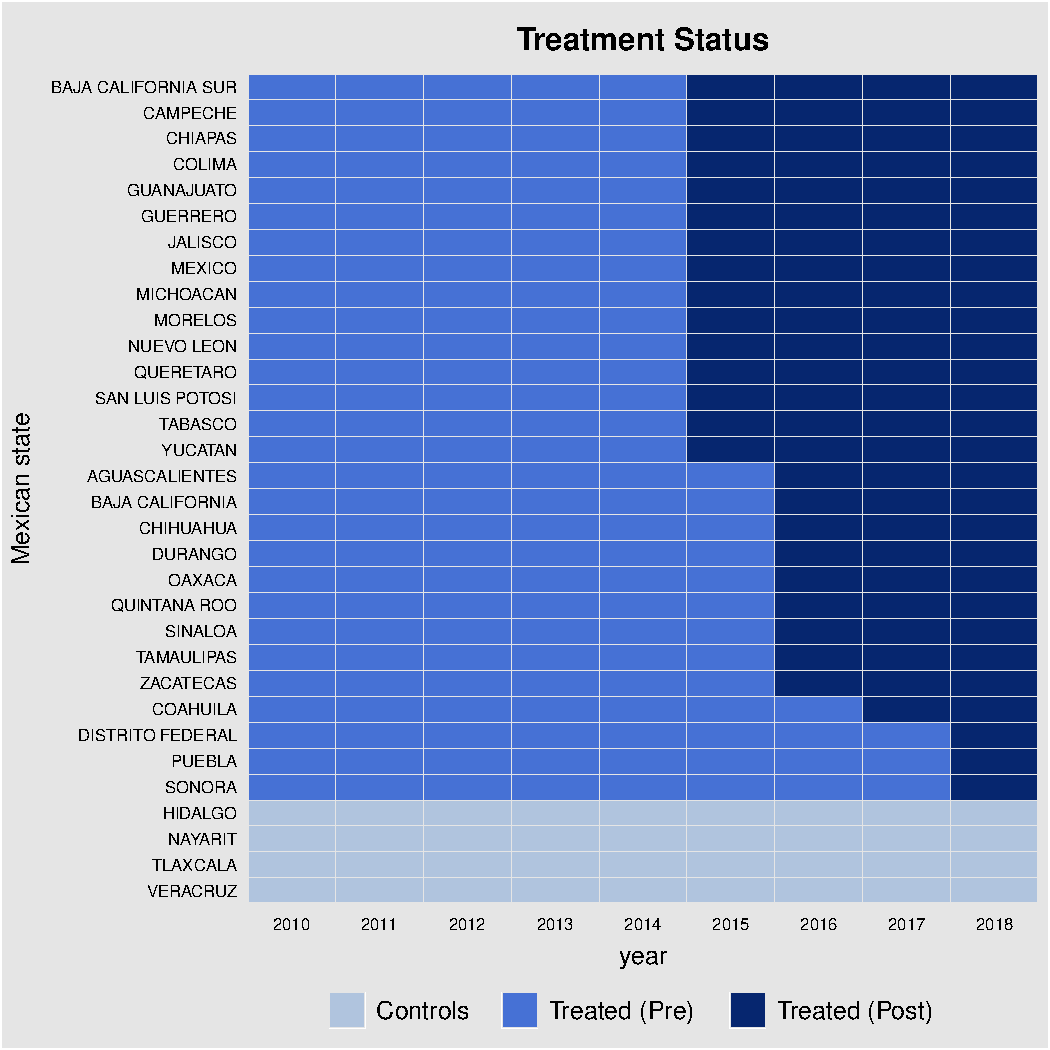
\includegraphics[width=0.75\textwidth]{Chapter2/Figures_incumbency/reform_treatmentstatus.pdf}     
\captionsetup{justification=centering} 
\end{figure}     
  
  
In regards to the implementation date, the Electoral Reform established that it would not affect any of the 2014 elections. Figure \ref{fig:treatment_status} describes the implementation period or treatment status of each of Mexico's 32 states.\footnote{Mexican states share the same administrative level as US states.} This figures allows to visualize the staggered rollout of the term limit removal. We have five timing groups: (1) 15 states who implemented reelection in 2015; (2) 9 who implemented reelection in 2016; (3) Coahuila who implemented reelection in 2017; (4) 4 states that implemented reelection in 2018; and (5) 4 states that will never be treated since they bypassed the reform by not allowing consecutive reelection (Hidalgo, Nayarit, Tlaxcala and Veracruz). Treatment in Figure \ref{fig:treatment_status} implies the following: Campeche, for example, begin treated starting in 2015 means that mayors elected in 2015 can run for reelection in the next election of 2018, as well as that of 2021 if they won in the previous one. Similarly, mayors in Chihuahua elected in 2016 can run for reelection in 2019, as well as 2022 since the reform allows mayors to reelect up to two consecutive terms. 

Evidence suggests that the differences in timing is a function of the staggered calendar of gubernatorial elections. As noted by \citet{motolinia_2020}, at the moment the reform was approved some governors were starting their terms while others were ending them. Those ending their terms had greater incentives to introduce reelection early on given that they could still apply political influence after leaving office by choosing people of their liking. In other words, governors influence in candidate selection of mayors seems to explain most of the variation in the staggered calendar of the implementation of the reform. For causal identification, it is important in empirical specifications to control for governors political power. 

\subsection{Empirical Specification} 
  
I estimate  a difference-in-discontinuity in close elections model that exploits the 2014 Electoral Reform that removed term limits for mayors in Mexico. To do so, I follow \citet{grembi_etal_2017} to estimate the boundary points of four regression functions of the probability of winning office (or the vote share) in the next election at $t+1$ ($Y_{m,t+1}$) on the winning margin of the election at $t$ for municipality $m$ and normalized at zero ($Margin_{m,t}$): two regressions on either side of the winning margin threshold (i.e., when $Margin_{m,t}$=0), before and after the implementation of the Term Limit Reform at $t_0$. Following \citet{gelman_imbens2014}, I fit a local linear regression for the observations distributed within an  \citet{calonicoetal_2014} optimal bandwidth distance $h$ to the forcing variable cutoff, for either side of $Margin_{m,t}$ before and after the implemenation of the Reform at $t_0$.\footnote{A rectangular kernel would give the same results as taking $E[Y]$ at a given bin on the distance to the cutting threshold. Other types of kernels, such as a triangular kernel, gives more weight to observations closer to the cutoff. I choose the latter for all estimations presented while estimations using a rectangular kernel are available upon request. Results are almost unchanged using the latter rather than the former.} In other words, I compare only municipalities in close elections and thus restrict the sample to those within a certain distance $h$ to the threshold, i.e. $Margin_{m,t} \in [Margin_{b-h}, Margin_{b+h}]$.  

The specification of the difference-in-discontinuity in close elections design is the following:

\begin{equation}
\small
\label{eq:abraham}
\begin{split}
Y_{m,t+1}=\mu_m + \lambda_t + \delta_1 f_{(.)}(VoteShareMargin)_{m,t} \\  
+ Win_{m,t}(\gamma_0 + \gamma_1 f_{(.)}(VoteShareMargin)_{m,t}) \\ + Reform_{m,t}[\alpha_o + \alpha_1f_{(.)}(VoteShareMargin)_{m,t} 
+ Win_{m,t}(\beta_0 + \beta_1 f_{(.)}(VoteShareMargin)_{m,t} )] \\ + \mathbf{X}_{s(m),t} \Phi + \epsilon_{m,t}
\end{split}
\end{equation}   

where $Y_{m,t+1}$ is either (a) a dummy=1 if party wins the following election at $t+1$, =0 otherwise, or (b) the vote share in election at $t+1$, 0 otherwise. $Win_{m,t}$ is a dummy=1 if an incumbent from $t-1$ barely lost the election at $t$, =0 if he lost. $Reform_{m,t}$ is a dummy=1 if a municipality implemented reelection for mayors, =0 otherwise, i.e. a post-treatment indicator. $f_{(.)}(VoteShareMargin)_{m,t}$ is the RD polynomial on winning margin for municipal election $m$ at calendar time $t$, having $f_{(.)}$ an \emph{n}th order polynomial of the forcing variable $VoteShareMargin_{m,t}$, which in this paper will be only a linear and quadratic polynomials.\footnote{Equation \ref{eq:abraham} shows the specification for the linear case. For the quadratic case, we would expand the equation to include all linear and quadratic polynomials interactions to have a fully saturated model.} $\mu_m$ and $\lambda_t$ are municipality and year fixed effects, with $\mathbf{X}_{s(m),t}$ a battery of controls including a dummy on the party alignment of the mayor with the governor, and the winning margin of the governor to proxy for governors influence in local politics. Standard errors are clustered at the state level as that is the level of treatment of the Electoral Reform in Mexico. 

The coefficient $\gamma_0$ is the regression discontinuity estimator that measures the incumbency returns for term-limited mayors. In other words, $\gamma_0$ captures the partisan incumbency advantage as term limited incumbents cannot run again for office but their parties can. The coefficient $\alpha_0$ is the difference-in-difference estimator on the effect of the Term Limit Reform on the probability of winning in the election at $t+1$. Conditional on municipal and period fixed effects, as well as other covariates, this estimator represents the difference in the probability of winning (or the vote share) in the next election $t+1$ for mayors without term limits to those with term limits. This coefficient does not measure an incumbency advantage. Lastly, the coefficient $\beta_0$ is the difference-in-discontinuity estimator that identifies the personal incumbency advantage by comparing municipalities where an incumbent barely wins an election to municipalities where an incumbent barely loses ($Win_{m,t}$), before and after term limit removal ($Reform_{m,t}$), i.e. the treatment $PersonalIncumbency_{m,t}=Reform_{m,t} \cdot Win_{m,t}$. Importantly, $\gamma_0$ and $\beta_0$ are divided by 2*Pr(Incumbent Runs Again) as some incumbents may retire in election $t$ as described in Section \ref{sec:design_literature}. 
 

\subsection{Data}  

The two main outcomes of interest are (i) an indicator of whether the incumbent party wins the mayoral office in election at $t+1$, and (ii) the vote share of the incumbent party in election at $t+1$. As described in the last section since the number of parties that compete for Mexican mayoral elections and win is large, I restrict the analysis only to incumbent parties following \citet{klasnja_titiunik_2017}. To do so, we need to identify a party that wins the election at $t-1$ and study the effects of this incumbent winning or losing at $t$ on the electoral outcomes (i) and (ii) at election $t+1$. For this we need at least three elections per municipality. The data covers all election years from 2006 to 2018. This allows to have at least two pre-reform election per municipality. 

For example, for the state of Michoacan we consider data for the elections of 2012 ($t-1$), 2015 ($t$) when the Electoral Reform was implemented, and 2018 ($t+1$). To check for pre-reform parallel trends we need additional elections prior to 2012. I include at least two full three-election cycles prior to treatment. Lets use the example of Michoacan again: the first cycle considers the election 2006 ($t-1$) to define the party that is the incumbent, who barely looses or wins at election at 2009 ($t$) on the electoral outcomes at the election at 2012 ($t+1$); the second cycle considers the election 2009 ($t-1$) to define the party that is the incumbent, who barely looses or wins at election at 2012 ($t$) on the electoral outcomes at the election at 2015 ($t+1$). To test for parallel trends we will only observe two coefficients prior to treatment of the incumbency advantage for the state of Michoacan: 2009 (as $t$ for the first cycle) on its effect on electoral outcomes at 2012 (as $t+1$ for the first cycle), and 2012 (as $t$ for the second cycle) on its effect on electoral outcomes at 2015 (as $t+1$ for the second cycle).   For other states these years may vary since each state holds different electoral calendars.\footnote{Municipal electoral calendars vary by state. However, almost all municipalities have three year terms with the exception of some municipalities with non-aligned electoral calendars with State-level ones, or other political circumstances.}

%However, since we generally have a reference period in event-study models, we do not show incumbency advantage results for the second cycle of 2012 (as $t$) and 2015 (as $t+1$).

To measure incumbent quality, I web-scraped professional titles and other characteristics for all municipal mayors in Mexico from 2010 to 2019 from the National Information Municipal System (SNIM for its abbreviation in Spanish). This novel database allows me to test for quality-based incumbency advantages.

I use several measures to proxy for the resources and effort placed by incumbents once in office. I use the National Institute of Statistics and Geography (INEGI for its acronym in Spanish) municipal level data on revenues and expenses from 2010 to 2018. I use data on total municipal revenues, as well as its subcomponents, specifically those coming from taxes, including property and estate taxes, as well as those from production, consumption and transaction taxes. These variables were deflated and are expressed in million pesos.\footnote{One dollar = 20 Mexican pesos approximately.} This data is further described in Section \ref{sec:mechanisms} while Appendix Table \ref{tab:descriptive} presents descriptive statistics.
  
\section{Main Results \label{sec:results}}

Table \ref{tab:naive_twfe} shows the $\gamma_0$ or coefficient of the partisan incumbency advantage, $\alpha_0$ or the coefficient of the difference in the probability of wining in the next election between term and non-term limited incumbents, and $\beta_0$ or the personal incumbency advantage. First, we observe that the introduction of reelection generated an incumbency \emph{advantage}, i.e. $\gamma_0 + \beta_0$ is equal to 4.5\% but not significant when using the probability of winning in the next election as outcome, and 4.6\% significant to the 1\% level for the linear specification. Results are similar for the quadratic polynomial specification. However, this positive incumbency advantage masks an asymmetry. First, we find a partisan incumbency \emph{disadvantage} of -5.38\% (not significant) in the probability of winning office in the next election, and a -3.32\% significant to the 1\% in the vote share in the next election [for the linear case and results are similar for the quadratic one]. These results are smaller than the ones identified in other Latin American cases like Brazil (-7.5\%), Colombia (-10\%) and Peru (-8.5\%) by \citet{klasnja_titiunik_2017}.\footnote{These numbers are the coefficients presented by \citet{klasnja_titiunik_2017} but divided by 2 and adjusted for the probability of running for office, a correction not done for these estimates.} 
 
\begin{table}[h]\def\sym#1{\ifmmode^{#1}\else\(^{#1}\)\fi}
\centering
\caption{Partisan and Personal Incumbency Advantage, Difference-in-Discontinuity of Close Elections Model}
\label{tab:naive_twfe}
\scalebox{0.75}{ 

\begin{tabular}{l*{4}{c}}
\hline \hline 
   
              &\multicolumn{2}{c}{\begin{tabular}[c]{@{}l@{}} Probability of winning, \\ Election at t+1\end{tabular}}&\multicolumn{2}{c}{\begin{tabular}[c]{@{}l@{}}  Vote Share,  \\ Election at t+1 \end{tabular}}\\\cmidrule(lr){2-3}\cmidrule(lr){4-5}
            &\multicolumn{1}{c}{(1)}         &\multicolumn{1}{c}{(2)}         &\multicolumn{1}{c}{(3)}         &\multicolumn{1}{c}{(4)}         \\
\addlinespace
Term Limit Reform ($\alpha\_0$)&      0.1780\sym{**} &      0.1789\sym{**} &      0.1656\sym{**} &      0.1656\sym{**} \\
            &    (0.0770)         &    (0.0770)         &    (0.0773)         &    (0.0771)         \\
\addlinespace
\begin{tabular}[c]{@{}l@{}} Dummy win, Election at t ($\gamma\_0$) \\ (Partisan Incumbency Advantage)\end{tabular}&     -0.0538         &     -0.0537         &     -0.0332\sym{***}&     -0.0332\sym{***}\\
            &    (0.0389)         &    (0.0392)         &    (0.0111)         &    (0.0110)         \\
\addlinespace
\begin{tabular}[c]{@{}l@{}} Interaction: Reform X Win Election at t ($\beta\_0$)  \\ (Personal Incumbency Advantage)\end{tabular}&      0.0986\sym{*}  &      0.0979         &      0.0788\sym{***}&      0.0787\sym{***}\\
            &    (0.0580)         &    (0.0591)         &    (0.0208)         &    (0.0209)         \\
\addlinespace
Observations&        2247         &        2247         &        1892         &        1892         \\
R-squared   &       0.535         &       0.535         &       0.558         &       0.558         \\
Municipal FE&  \checkmark         &  \checkmark         &  \checkmark         &  \checkmark         \\
Year FE     &  \checkmark         &  \checkmark         &  \checkmark         &  \checkmark         \\
Controls$^a$&                     &                     &                     &                     \\
Polynomial  &      linear         &   quadratic         &      linear         &   quadratic         \\
Incumbency Advantage: Partisan ($\gamma\_0$) + Personal($\beta\_0$)&  $0.045^{}$         &  $0.044^{}$         &$0.046^{***}$         &$0.045^{***}$         \\
SE(Incumbency Advantage)&       0.036         &       0.036         &       0.017         &       0.017         \\
Difference:Personal($\beta\_0$)-Partisan($\gamma\_0$)& $0.1523^{}$         & $0.1516^{}$         &$0.1119^{***}$         &$0.1119^{***}$         \\
SE(Difference)&      0.0919         &      0.0935         &      0.0289         &      0.0290         \\
   
     
      
\hline \hline 
\multicolumn{5}{p{1.2\textwidth}}{\footnotesize{Notes: Standard errors in parentheses are clustered at the state level. Significance-level: $^{***}$ 1\%; $^{**}$ 5\%; and $^*$ 10\%, that refer to two-sided t-test.$^a$ Pretreatment controls include: governor winning margin; party alignment with the President;  party alignment with the Governor; and logged population.}} \\
\end{tabular}
}
\end{table}    


Second, we observe a personal incumbency \emph{advantage} of 9.86\% significant to the 10\% in the probability of winning office, and of 7.88\% significant to the 1\% level for vote share in the next election [for the linear case and results are similar for the quadratic one]. The personal incumbency advantage found is not small representing almost half a standard deviation for the vote share, and a quarter of a standard deviation for the probability of winning office in the next election. Interestingly, the personal incumbency advantage is similar to the one find by \citet{fowler_hall_2014} for the case of the US of 8.8\%. They also find a negative partisan incumbency of -2\% but not significant.  

Table \ref{tab:naive_twfe} shows that prior to the introduction of the Electoral Reform Mexico's mayoral elections showed an incumbency disadvantage (a partisan one since their where term limits). This result has been confirmed by \citet{klasnja_titiunik_2017} who run a regression discontinuity design for close elections considering all elections from 1997 to 2009 in Mexico. However, once reelection is introduced a decrease in the incumbency disadvantage is observed and as noted in Table \ref{tab:naive_twfe} it even became positive and not different from zero. This decay in the incumbency disadvantage with the removal of term limits is similar to the finding by \citet{klasnja_titiunik_2017} when comparing the incumbency returns from countries with term limits -mainly Brazil, Mexico, and Colombia-  to those with indefinite reelection -Peru, Chile and Costa Rica: while the former show an average incumbency disadvantage of -19\% (significant to the 1\% level) in the probability of winning office the latter show an incumbency disadvantage of -2\% (non-significant). In the case of \citet{klasnja_titiunik_2017} they believe incumbency disadvantage is explained by voters blaming weak parties from not being able to sanction their members from undesirable behavior in office, specially when they are term limited and there is no need to be responsive for voters. They mention that the removal of term limits could have strengthen the accountability between voters and representatives which should decrease the responsibility put on parties to control their members decreasing the incumbency disadvantage. The asymmetry found in Table \ref{tab:naive_twfe} offers a closely related logic: reelection creates an ``electoral connection'' between voters and incumbents \citep{mayhew_1974}; as a result, a personal incumbency advantage is created signaling that voters believe incumbents and not their parties are responsible for policy actions. In other words, a personal incumbency advantage is the main driver in the decrease in incumbency disadvantage in Mexico, and plausibly other countries too. Moreover, this result speaks to a potential party dealignment in Mexican politics after the introduction of reelection. Not only has the country experienced a decrease in winning margins and various changes in party bases in the last two decades, but citizens at the municipal level are associating policy actions to representatives rather than their parties.   


Lastly, it is important to notice that mayors up for reelection had a higher probability of winning office in the next election relative to term-limited mayors whose parties will run again. This is not a measure of incumbency advantage but just a difference in the probability of winning office. The probability is not small, however, it represents a greater likelihood of 17.8\% significant to the 5\% level of winning office in the next election, and a greater vote share of 16.6\% in the next election. 
   
\subsection{Identification assumptions} 

To validate causal effects three identification assumptions need to hold. First, parallel trends for both incumbency advantage measures need to hold. As seen in Figure \ref{fig:event_study_personal}  this is the case for both the probability of winning and vote share at election $t+1$. This Figure shows an event study design of the same data used to estimate Table \ref{tab:naive_twfe} but constructing $t$ year indicators relative to treatment implementation. The period $t=0$ represents the year in which the Electoral Reform was implemented. Periods prior to $t=0$ speak to the years prior to the implementation of the reform. For example, $t-6$ represents two election cycles prior to $t=0$ since for some municipalities electoral cycles last 3 years.  $t-5$ and $t-4$ also represent two election cycles prior to the implementation of the reform at $t$ but for municipalities where their calendars gave only 2 or 1 years for mayors in office, which corresponds to states that where aligning their municipal and gubernatorial calendars (E.g., Puebla). Figure \ref{fig:event_study_personal} omits the election prior to the implementation of the Reform to serve as comparison group: these is the period three years prior to $t=0$, i.e. $t-3$. There were no elections in years $t-2$ and $t-1$. Thus, estimated coefficients are interpreted as the difference relative to the election prior to the implementation of the Reform.\footnote{Potential treatment effect heterogeneity of the different treatment cohorts of the Reform may introduce bias to the difference-in-discontinuity estimators. I follow \citet{abraham_sun_2020} and run a cohort weighted event study design that takes into account treatment effect heterogeneity. Results show parallel trends and similar results to those of  Figure \ref{fig:event_study_personal}. Results available upon request.} Figure \ref{fig:event_study_personal} shows the difference-in-discontinuity estimator $\beta_0$, i.e. the personal incumbency advantage before and after the implementation of the Reform. Parallel trends are found for both the linear and quadratic polynomial specifications.  

Second, no anticipatory behavior from municipalities should be found; since we are only taking into account one election cycle post-treatment, we don't anticipate incumbents reacting in such a short time window. Third, the design would be invalid if parties could manipulate close elections and sort themselves to those that imply a higher probability of winning. Two tests are commonly used to show validity on the design: (a) no covariate jump at the discontinuity on relevant pre-treatment variables and (b) density tests to see whether the number of municipalities above (or below) the cutoff threshold is significantly different from the number of municipalities below (or above). Appendix Figure \ref{fig:jump_covariates} shows evidence of no significant jump at the discontinuity of various pretreatment covariates including a dummy on the alignment with the president, alignment with the governor, logged population, a dummy of the party who was ruling the municipality one election before (PRI, PAN or MORENA/PRD), and the effective number of parties. Furthermore, Appendix Figure \ref{fig:mccrary} shows no density difference between municipalities just above and below the winning margin cutoff ($Margin_{m,t}=0$) for the linear and polynomial specifications. 

\begin{figure}[H]   
\centering    
 \caption{Event Study: Personal Incumbency Advantage}
 \label{fig:event_study_personal}
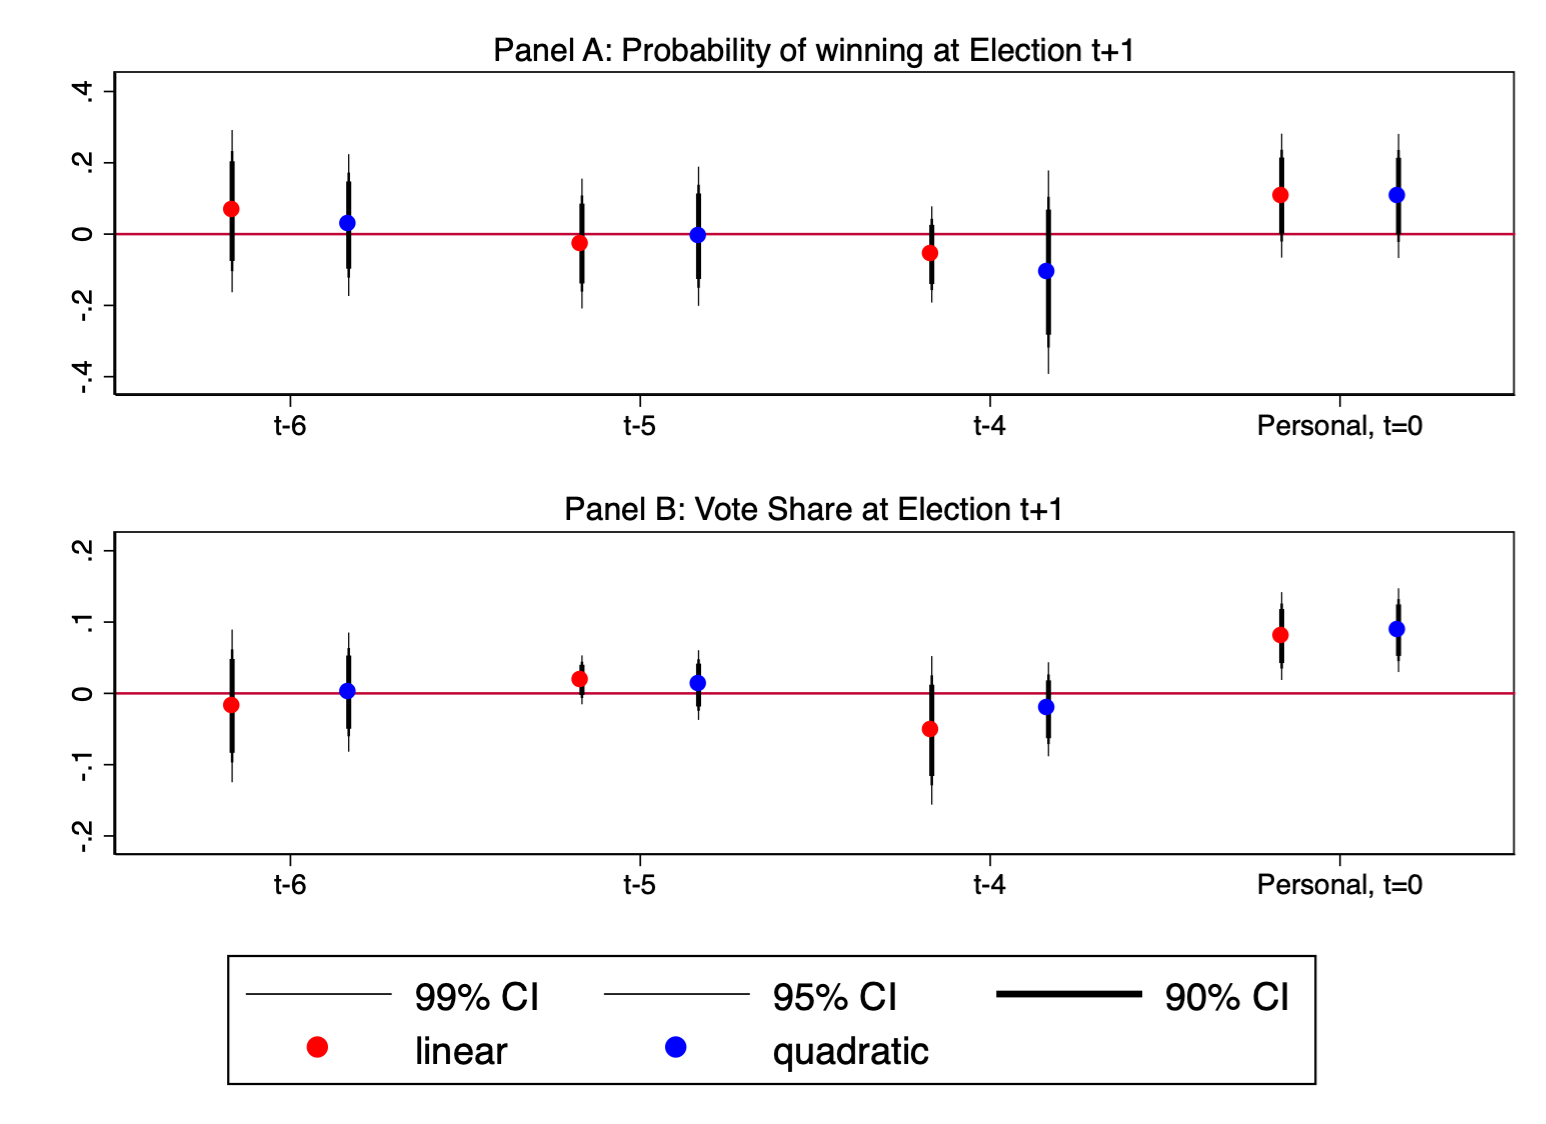
\includegraphics[width=0.9\textwidth]{Chapter2/Figures_incumbency/event_study.png}
       \captionsetup{justification=centering}
         
 \textbf{Note:} Figure \ref{fig:event_study_personal} shows the average difference-in-discontinuity estimator of the effect of the Term Limit Reform that compares municipalities with incumbents that barely won to those that barely lost in the election at $t$ on the probability of winning in the election at $t+1$ (Panel A) and the vote share in the  election at $t+1$ (Panel B). Optimal bandwidths following \citet{calonicoetal_2014} are used. 
  
\end{figure}  
 
    
\subsection{Robustness tests \label{sec:robustness}} 
  
To test the robustness of results I start by comparing the difference-in-discontinuity of close election design results from Table \ref{tab:naive_twfe} with the design used by \citet{fowler_hall_2014}. To estimate the personal and partisan incumbency advantages \citet{fowler_hall_2014} run two different regressions: first, a regression discontinuity design of close elections where candidates are prevented from running for reelection, i.e. they are term limited; second, a regression discontinuity design where candidates are non-term limited, i.e. they can run for reelection if desired. The difference between the estimated coefficients of these two models results in the personal incumbency advantage, while the first one estimates the partisan one and the second one the conjoint partisan and personal incumbency advantages. Results are then corrected by the probabilities of reelection attempts as described in Section \ref{sec:design_literature}. Table \ref{tab:fowler_hall} shows the partisan and personal incumbency advantages following \citet{fowler_hall_2014} using both the probability of victory as well as the winning margin in the next election as outcomes, and all mayoral elections in Mexico since 2000. Panel A shows the results using a linear polynomial while Panel B uses a quadratic one. Overall, we see that without term limits, in Mexico incumbents had a positive but non-significant incumbency advantage. However, term limited races show that a partisan incumbency disadvantage exists between -8 to -9\% depending on the specification. Contrastingly, the difference between the term limit and non-term limit cases in column (3) shows the personal incumbency returns to be positive and significant to the 1\% level. These results coincide with the asymmetry found in Table \ref{tab:naive_twfe}. The difference with the results from Table \ref{tab:naive_twfe}, however, is that for the results of Table \ref{tab:fowler_hall} to be identified we need to assume parallel trends hold.   

\begin{table}[htbp]\def\sym#1{\ifmmode^{#1}\else\(^{#1}\)\fi}
\centering
\caption{Personal and Partisan Incumbency Advantage following \citet{fowler_hall_2014}}
\label{tab:fowler_hall}
\scalebox{1}{
\begin{tabular}{lccc}
\hline \hline
& \multicolumn{3}{c}{\textbf{Panel A: linear polynomial}}\\
& \multicolumn{1}{c}{No term limits:} & \multicolumn{1}{c}{term limits:} & \multicolumn{1}{c}{difference:}\\
Advantage: & \multicolumn{1}{c}{personal + partisan} & \multicolumn{1}{c}{partisan} & \multicolumn{1}{c}{personal} \\
& \multicolumn{1}{c}{(1)} & \multicolumn{1}{c}{(2)} & \multicolumn{1}{c}{(3)} \\
\cmidrule(lrr){2-2}  \cmidrule(lrr){3-3} \cmidrule(lrr){4-4}\\
\addlinespace
RD estimate: prob(victory in t+1) &      $ 0.0568^{} $ &  $ -0.1269^{***} $  &  $ 0.1468^{***} $  \\
& ($ 0.0508$) & ($ 0.0208 $)  & ($ 0.0038 $)\\
RD estimate: vote share in t+1 &      $ 0.0245^{} $ &  $ -0.0529^{***} $  &  $ 0.0618^{***} $  \\
& ($ 0.0243$) & ($ 0.0073 $)  & ($ 0.0024 $)\\
\addlinespace
Observations: prob(victory in t+1)      &            1257        &     9180  \\
Observations: vote share in t+1      &            1221        &     8758  \\
\\
& \multicolumn{3}{c}{\textbf{Panel B: quadratic polynomial}}\\
& \multicolumn{1}{c}{No term limits:} & \multicolumn{1}{c}{term limits:} & \multicolumn{1}{c}{difference:}\\
Advantage: & \multicolumn{1}{c}{personal + partisan} & \multicolumn{1}{c}{partisan} & \multicolumn{1}{c}{personal} \\
& \multicolumn{1}{c}{(1)} & \multicolumn{1}{c}{(2)} & \multicolumn{1}{c}{(3)} \\
\cmidrule(lrr){2-2}  \cmidrule(lrr){3-3} \cmidrule(lrr){4-4}\\
\addlinespace
RD estimate: prob(victory in t+1) &      $ 0.0442^{} $ &  $ -0.1291^{***} $  &  $ 0.1384^{***} $  \\
& ($ 0.0676$) & ($ 0.0258 $)  & ($ 0.0042 $)\\
RD estimate: vote share in t+1 &      $ 0.0311^{} $ &  $ -0.0510^{***} $  &  $ 0.0656^{***} $  \\
& ($ 0.0274$) & ($ 0.0092 $)  & ($ 0.0026 $)\\
\addlinespace
Observations: prob(victory in t+1)      &            1257        &     9180  \\
Observations: vote share in t+1      &            1221        &     8758  \\
\hline \hline
\multicolumn{4}{p{1\textwidth}}{\footnotesize{Notes: Standard errors in parentheses are clustered at the state level, with the following significance-level: $^{***}$ 1\%; $^{**}$ 5\%; and $^*$ 10\%, that refer to two-sided t-test with the null hypothesis equal to 0 for each relative time period. Table estimated using all elections since the year 2000.}}
\end{tabular}
}
\end{table}
   


For robustness we also check whether results change by varying the bandwidth for close elections. Appendix Figure \ref{fig:bandwidths} shows this to be the case overall, with an asymmetry found between the partisan and personal incumbency advantages for the linear and quadratic specifications, using both the probability of winning or vote share in the election $t+1$.       


\section{Mechanisms: What explains the observed electoral returns from incumbency? \label{sec:mechanisms}}
           
A big concern of the literature has been understanding the determinants of incumbency advantage. To date, we can identify at least three broad types of explanations. First, what incumbents do (and opponents cannot do) emphasizing the resources, visibility, and power that incumbents gain from office holding \citep{mayhew_1974, fiorina_1989, king_1991, cox_morgensten_1993}.  Second, quality-based explanations that emphasize who incumbents are (and who their opponents are) \citep{cox_katz_1996, levitt_wolfram_1997, ansolabehere_snyder_2000, eggers_2017}. In this second line we find explanations related to incumbents’ quality as well as the “scare-off effect”, or the ability incumbents have to scare off high-quality challengers. A third and more recent type of mechanism emphasizes the role of information. \citet{ashworth_bdm_2008} find that incumbency advantage is dependent on how precise the information is about incumbent’s ability to voters. More recently, \citet{ashworth_etal_2019} expand on the role of information to explain incumbency advantage: through a theoretical model, they show that incumbents have an additional information advantage to challengers: they govern while challengers do not. This is so even absent any partisanship, electoral selection or challenger scare off. However, to date there is no empirical identification of the information-based explanation proposed by these authors. Moreover, if theoretical work done by Ashworth and co-authors is correct, all other explanations of incumbency advantage might be biased by the role information plays. 
 
To test if a resource-based incumbency advantage explains the returns observed in Section \ref{sec:results}, I evaluate the effect of the reform on municipal revenues and fiscal transfers. Local tax revenues have been used by the incumbency advantage literature to test whether a resourced-based incumbency advantage exists \citep{fiorina_1989, cox_morgensten_1993}. The most relevant tax revenues at the municipal level in Mexico are property and estate taxes. Two additional sources of local revenues are important, those coming from the ownership of vehicles (\emph{tenencia} in Spanish) as well as revenues from taxing new cars. Mayors tend to use these two sources of revenues to increase their treasury but are highly unapproved by voters. As a result, we would expect mayors with reelection incentives not to rely on these types of tax revenues. Table \ref{tab:revenues} Panel A shows that total municipal revenues increased by 44 million pesos significant to the 5\% level for mayors up for reelection and that barely won in the election at $t$ relative to those with term limits and barely lost at $t$.  This is true for the linear and quadratic specifications.\footnote{One dollar is equivalent to 20 pesos approximately.} This result represents an increase of a quarter of the mean of total municipal revenues. A large increase of municipal revenues comes from an increase in tax revenues (columns 3 and 4 of Panel A), particularly property tax revenues (columns 5 and 6), and estate tax revenues (columns 7 and 8). Null effects are found for production, consumption and transactions tax revenues in Panel B columns 1 and 2. Interestingly, unpopular taxes like the \emph{tenencia} decrease in revenues for mayors up for reelection and that barely won in election $t$ relative to those term limited and that barely lost in $t$. Now, the increase in municipal revenues is used as a measure of the increase in resources. The increase could be driven by an increase in the effort of tax collection, an increase in tax rates or better economic conditions that lead to higher tax revenues. For the case of municipal revenues in Mexico it is hard to disentangle between these three mechanisms, specially since there is no data on local tax rates or effort in tax collection. The main takeaway, however, is that municipalities with mayors up for reelection at that barely won their election at $t$ increase the amount of resources. As a result, voters create a resource-based incumbency advantage with the believe that they will receive a higher budget or transfer in the future. %%%rewrite .

 %\begin{landscape} 
 %REVENUES     
\begin{table}[htbp]\def\sym#1{\ifmmode^{#1}\else\(^{#1}\)\fi}
\centering
\caption{Revenues of Municipal Governments, Difference-in-Discontinuity of Close Elections Model}
\label{tab:revenues}
\scalebox{0.55}{ 
\begin{tabular}{l*{8}{c}}
\hline \hline 
\\
& \multicolumn{8}{c}{\textbf{Panel A:}}  \\


Dependent variable in million pesos$^b$: & \multicolumn{2}{c}{\begin{tabular}[c]{@{}c@{}}Total Municipal \\ Revenues\end{tabular}}  & \multicolumn{2}{c}{Tax Revenues} & \multicolumn{2}{c}{\begin{tabular}[c]{@{}c@{}}Property Tax \\ Revenues\end{tabular}} & \multicolumn{2}{c}{\begin{tabular}[c]{@{}c@{}}Estate Tax \\ Revenues\end{tabular}} \\
\cmidrule(lr){2-3}\cmidrule(lr){4-5}\cmidrule(lr){6-7}\cmidrule(lr){8-9}


             &\multicolumn{1}{c}{linear}&\multicolumn{1}{c}{quadratic}&\multicolumn{1}{c}{linear}&\multicolumn{1}{c}{quadratic}&\multicolumn{1}{c}{linear}&\multicolumn{1}{c}{quadratic}&\multicolumn{1}{c}{linear}&\multicolumn{1}{c}{quadratic}\\\cmidrule(lr){2-2}\cmidrule(lr){3-3}\cmidrule(lr){4-4}\cmidrule(lr){5-5}\cmidrule(lr){6-6}\cmidrule(lr){7-7}\cmidrule(lr){8-8}\cmidrule(lr){9-9}
            &\multicolumn{1}{c}{(1)}         &\multicolumn{1}{c}{(2)}         &\multicolumn{1}{c}{(3)}         &\multicolumn{1}{c}{(4)}         &\multicolumn{1}{c}{(5)}         &\multicolumn{1}{c}{(6)}         &\multicolumn{1}{c}{(7)}         &\multicolumn{1}{c}{(8)}         \\
\addlinespace
Term Limit Reform&    -32.2546\sym{***}&    -31.5521\sym{***}&      0.7710         &      0.8451         &      2.8797         &      3.0528         &     -1.5350         &     -1.4900         \\
            &   (10.0656)         &   (10.4937)         &    (2.8949)         &    (2.9493)         &    (2.4988)         &    (2.5249)         &    (2.7821)         &    (2.8250)         \\
\addlinespace
\begin{tabular}[c]{@{}l@{}} Dummy win, Election at t \end{tabular}&    -15.2045         &    -14.4905         &     -0.8681         &     -0.7554         &     -3.6883\sym{*}  &     -3.5814         &     -3.6395         &     -3.5547         \\
            &    (9.5364)         &    (8.9873)         &    (2.3791)         &    (2.4264)         &    (2.1232)         &    (2.1299)         &    (2.2483)         &    (2.2599)         \\
\addlinespace
\begin{tabular}[c]{@{}l@{}} Interaction: Reform X Win Election at t \end{tabular}&     44.2806\sym{**} &     44.9223\sym{**} &      7.1171\sym{**} &      7.4166\sym{**} &      6.3265\sym{**} &      6.4784\sym{**} &      9.2480\sym{**} &      9.3405\sym{**} \\
            &   (16.0947)         &   (16.3556)         &    (2.7790)         &    (2.8267)         &    (2.8047)         &    (2.8943)         &    (3.4478)         &    (3.5175)         \\
\addlinespace
Observations&        1352         &        1352         &        1366         &        1366         &         984         &         984         &        1170         &        1170         \\
R-squared   &       0.981         &       0.981         &       0.967         &       0.967         &       0.964         &       0.964         &       0.971         &       0.971         \\
Municipal FE&  \checkmark         &  \checkmark         &  \checkmark         &  \checkmark         &  \checkmark         &  \checkmark         &  \checkmark         &  \checkmark         \\
Year FE     &  \checkmark         &  \checkmark         &  \checkmark         &  \checkmark         &  \checkmark         &  \checkmark         &  \checkmark         &  \checkmark         \\
Controls$^a$&                     &                     &                     &                     &                     &                     &                     &                     \\
Polynomial  &      linear         &   quadratic         &      linear         &   quadratic         &      linear         &   quadratic         &      linear         &   quadratic         \\
Difference:Personal($\beta\_0$)-Partisan($\gamma\_0$)&$59.4850^{**}$         &$59.4128^{**}$         &$7.9852^{*}$         &$8.1720^{*}$         &$10.0149^{**}$         &$10.0599^{**}$         &$12.8876^{**}$         &$12.8952^{**}$         \\
SE (Difference)&     23.5860         &     23.3221         &      4.1091         &      4.0936         &      3.7193         &      3.7970         &      5.3087         &      5.3617         \\
Mean DV in million pesos$^b$&       190.6         &       190.6         &        23.3         &        23.3         &        15.0         &        15.0         &        21.4         &        21.4         \\
   
   
\\
& \multicolumn{8}{c}{\textbf{Panel B:}}  \\
\\
Dependent variable in million pesos$^b$: & \multicolumn{2}{c}{\begin{tabular}[c]{@{}c@{}}Prod., Cons. and \\ Trans. Tax Revenues \end{tabular}} & \multicolumn{2}{c}{\begin{tabular}[c]{@{}c@{}}Vehicle Ownership Tax \\ Revenues (\emph{Tenencia}) \end{tabular}}  & \multicolumn{2}{c}{\begin{tabular}[c]{@{}c@{}}New Cars Tax \\ Revenues \end{tabular}} \\
 \cmidrule(lr){2-3}\cmidrule(lr){4-5}\cmidrule(lr){6-7}

             &\multicolumn{1}{c}{linear}&\multicolumn{1}{c}{quadratic}&\multicolumn{1}{c}{linear}&\multicolumn{1}{c}{quadratic}&\multicolumn{1}{c}{linear}&\multicolumn{1}{c}{quadratic}\\\cmidrule(lr){2-2}\cmidrule(lr){3-3}\cmidrule(lr){4-4}\cmidrule(lr){5-5}\cmidrule(lr){6-6}\cmidrule(lr){7-7}
            &\multicolumn{1}{c}{(1)}         &\multicolumn{1}{c}{(2)}         &\multicolumn{1}{c}{(3)}         &\multicolumn{1}{c}{(4)}         &\multicolumn{1}{c}{(5)}         &\multicolumn{1}{c}{(6)}         \\
\addlinespace
Term Limit Reform&      6.8810         &      6.9335         &     -0.3763         &     -0.3717         &      0.1546\sym{**} &      0.1594\sym{**} \\
            &    (6.8291)         &    (6.8923)         &    (0.2705)         &    (0.2726)         &    (0.0723)         &    (0.0740)         \\
\addlinespace
\begin{tabular}[c]{@{}l@{}} Dummy win, Election at t \end{tabular}&      8.5129         &      8.5019         &      0.2589         &      0.2554         &     -0.0630         &     -0.0648         \\
            &    (9.0537)         &    (9.0607)         &    (0.1999)         &    (0.2046)         &    (0.1189)         &    (0.1203)         \\
\addlinespace
\begin{tabular}[c]{@{}l@{}} Interaction: Reform X Win Election at t \end{tabular}&     -8.6016         &     -8.5001         &     -1.0651\sym{**} &     -1.0659\sym{**} &      0.2978\sym{*}  &      0.2957\sym{*}  \\
            &    (8.8616)         &    (8.7694)         &    (0.4581)         &    (0.4602)         &    (0.1628)         &    (0.1606)         \\
\addlinespace
Observations&         409         &         409         &        1043         &        1043         &        1317         &        1317         \\
R-squared   &       0.521         &       0.521         &       0.658         &       0.658         &       0.969         &       0.969         \\
Municipal FE&  \checkmark         &  \checkmark         &  \checkmark         &  \checkmark         &  \checkmark         &  \checkmark         \\
Year FE     &  \checkmark         &  \checkmark         &  \checkmark         &  \checkmark         &  \checkmark         &  \checkmark         \\
Controls$^a$&                     &                     &                     &                     &                     &                     \\
Polynomial  &      linear         &   quadratic         &      linear         &   quadratic         &      linear         &   quadratic         \\
Difference:Personal($\beta\_0$)-Partisan($\gamma\_0$)&$-17.1145^{}$         &$-17.0020^{}$         &$-1.3240^{**}$         &$-1.3212^{**}$         & $0.3608^{}$         & $0.3605^{}$         \\
SE (Difference)&     17.8925         &     17.8078         &      0.6052         &      0.6123         &      0.2718         &      0.2703         \\
Mean DV in million pesos$^b$&         1.6         &         1.6         &         0.6         &         0.6         &         0.9         &         0.9         \\
   
    
        
\hline \hline 
\multicolumn{9}{p{1.6\textwidth}}{\footnotesize{Notes: Standard errors in parentheses are clustered at the state level. Significance-level: $^{***}$ 1\%; $^{**}$ 5\%; and $^*$ 10\%, that refer to two-sided t-test.$^a$ Pretreatment controls include: governor winning margin; party alignment with the President;  party alignment with the Governor; and logged population. $^b$ 1 dollar = 20 pesos approximately. Thus, 1 million pesos are \$200,000 USD.}} \\
\end{tabular}
}.  
\end{table}    
%\end{landscape}   
        

 Besides revenues, we can use data on municipal transfers from the federation or the state to proxy for resources. These transfers can be divided into two types: ear-marked and not ear-marked. Ear-marked transfers are those which are determined mostly by the use of fiscal formulas and are targeted to specific ``ear-marked'' expenses or conditional on certain activities. The most prominent municipal transfer in Mexico are the Federal and State Contributions Fund. Not ear-marked transfers are those that municipalities can exercise freely and are generally not audited by Federal Superior Audit in Mexico. The most prominent ones include the General Participation Fund as well as secondary participating funds. Other not ear-marked municipal transfers are the Municipal Development Fund, the Contribution Fund to Strengthen Municipalities and the Contribution Fund for Municipal Social Infrastructure. Table \ref{tab:transfers} shows the effect of the Term Limit Reform on these transfers. We see an increase of participations (columns 1-4 in Panel A), as well as contributions to municipal social infrastructure (columns 3 and 4 in Panel B)  in municipalities where mayors can run for reelection and barely won in election $t$ relative to those that are term limited and barely lost in election $t$. In contrast, no effects are found for ear-marked transfers, mainly the Federal and State Contributions. 
   
        
 %\begin{landscape}  
 %TRANSFERS    
\begin{table}[htbp]\def\sym#1{\ifmmode^{#1}\else\(^{#1}\)\fi}
\centering
\caption{Transfers to Municipal Governments from the Federation and the State, Difference-in-Discontinuity of Close Elections Model}
\label{tab:transfers}
\scalebox{0.6}{ 
\begin{tabular}{l*{6}{c}}
\hline \hline 
\\
& \multicolumn{6}{c}{\textbf{Panel A:}}  \\

        
Dependent variable in million pesos$^b$: & \multicolumn{2}{c}{\begin{tabular}[c]{@{}c@{}}General Participation \\ Fund\end{tabular}}  & \multicolumn{2}{c}{Participating Funds} & \multicolumn{2}{c}{\begin{tabular}[c]{@{}c@{}}Municipal Development \\ Fund\end{tabular}}  \\
\cmidrule(lr){2-3}\cmidrule(lr){4-5}\cmidrule(lr){6-7}
             &\multicolumn{1}{c}{linear}&\multicolumn{1}{c}{quadratic}&\multicolumn{1}{c}{linear}&\multicolumn{1}{c}{quadratic}&\multicolumn{1}{c}{linear}&\multicolumn{1}{c}{quadratic}\\\cmidrule(lr){2-2}\cmidrule(lr){3-3}\cmidrule(lr){4-4}\cmidrule(lr){5-5}\cmidrule(lr){6-6}\cmidrule(lr){7-7}
            &\multicolumn{1}{c}{(1)}         &\multicolumn{1}{c}{(2)}         &\multicolumn{1}{c}{(3)}         &\multicolumn{1}{c}{(4)}         &\multicolumn{1}{c}{(5)}         &\multicolumn{1}{c}{(6)}         \\
\addlinespace
Term Limit Reform&     -3.7726         &     -3.7781         &     -0.1525         &      0.0139         &      0.2237         &      0.2140         \\
            &    (3.1636)         &    (3.1626)         &    (3.2576)         &    (3.3629)         &    (0.4757)         &    (0.4772)         \\
\addlinespace
\begin{tabular}[c]{@{}l@{}} Dummy win, Election at t \end{tabular}&     -0.6749         &     -0.6681         &      0.4634         &      0.6110         &      0.0366         &      0.0509         \\
            &    (2.2195)         &    (2.2276)         &    (2.7421)         &    (2.7506)         &    (0.5091)         &    (0.5186)         \\
\addlinespace
\begin{tabular}[c]{@{}l@{}} Interaction: Reform X Win Election at t \end{tabular}&      6.6213\sym{**} &      6.6825\sym{**} &      8.0174\sym{**} &      8.3615\sym{**} &      0.8701         &      0.8906         \\
            &    (2.8621)         &    (2.7983)         &    (3.3955)         &    (3.4249)         &    (0.6735)         &    (0.6753)         \\
\addlinespace
Observations&        1317         &        1317         &        1285         &        1285         &        1138         &        1138         \\
R-squared   &       0.981         &       0.981         &       0.976         &       0.976         &       0.986         &       0.986         \\
Municipal FE&  \checkmark         &  \checkmark         &  \checkmark         &  \checkmark         &  \checkmark         &  \checkmark         \\
Year FE     &  \checkmark         &  \checkmark         &  \checkmark         &  \checkmark         &  \checkmark         &  \checkmark         \\
Controls$^a$&                     &                     &                     &                     &                     &                     \\
Polynomial  &      linear         &   quadratic         &      linear         &   quadratic         &      linear         &   quadratic         \\
Difference:Personal($\beta\_0$)-Partisan($\gamma\_0$)& $7.2962^{}$         & $7.3506^{}$         & $7.5540^{}$         & $7.7505^{}$         & $0.8335^{}$         & $0.8397^{}$         \\
SE (Difference)&      4.5115         &      4.4352         &      4.9473         &      4.9230         &      0.9980         &      1.0088         \\
Mean DV in million pesos$^b$&        41.5         &        41.5         &        54.7         &        54.7         &        10.0         &        10.0         \\
   

\\
& \multicolumn{6}{c}{\textbf{Panel B:}}  \\
\\
Dependent variable in million pesos$^b$: & \multicolumn{2}{c}{\begin{tabular}[c]{@{}c@{}}Contributions Fund to \\ Strengthen Municipalities \end{tabular}} & \multicolumn{2}{c}{\begin{tabular}[c]{@{}c@{}}Contribution Fund for \\ Municipal Social Infrastructure \end{tabular}}  & \multicolumn{2}{c}{\begin{tabular}[c]{@{}c@{}}Federal and State \\ Contributions \end{tabular}} \\
 \cmidrule(lr){2-3}\cmidrule(lr){4-5}\cmidrule(lr){6-7}

             &\multicolumn{1}{c}{linear}&\multicolumn{1}{c}{quadratic}&\multicolumn{1}{c}{linear}&\multicolumn{1}{c}{quadratic}&\multicolumn{1}{c}{linear}&\multicolumn{1}{c}{quadratic}\\\cmidrule(lr){2-2}\cmidrule(lr){3-3}\cmidrule(lr){4-4}\cmidrule(lr){5-5}\cmidrule(lr){6-6}\cmidrule(lr){7-7}
            &\multicolumn{1}{c}{(1)}         &\multicolumn{1}{c}{(2)}         &\multicolumn{1}{c}{(3)}         &\multicolumn{1}{c}{(4)}         &\multicolumn{1}{c}{(5)}         &\multicolumn{1}{c}{(6)}         \\
\addlinespace
Term Limit Reform&     -0.7954         &     -0.7805         &      0.7868         &      0.8159         &    -16.8333\sym{**} &    -16.5883\sym{**} \\
            &    (1.4516)         &    (1.4718)         &    (1.4226)         &    (1.3971)         &    (6.6819)         &    (6.7282)         \\
\addlinespace
\begin{tabular}[c]{@{}l@{}} Dummy win, Election at t \end{tabular}&     -0.0917         &     -0.0267         &     -1.4125         &     -1.4166         &     -3.9379         &     -3.8393         \\
            &    (1.0806)         &    (1.1145)         &    (1.7105)         &    (1.7182)         &    (4.4769)         &    (4.4217)         \\
\addlinespace
\begin{tabular}[c]{@{}l@{}} Interaction: Reform X Win Election at t \end{tabular}&      1.1915         &      1.2527         &      2.9133\sym{**} &      2.8935\sym{**} &     21.9864         &     22.1860         \\
            &    (1.9003)         &    (1.8980)         &    (1.4145)         &    (1.4071)         &   (13.0689)         &   (13.1533)         \\
\addlinespace
Observations&        1264         &        1264         &        1554         &        1554         &        1367         &        1367         \\
R-squared   &       0.980         &       0.980         &       0.881         &       0.881         &       0.894         &       0.894         \\
Municipal FE&  \checkmark         &  \checkmark         &  \checkmark         &  \checkmark         &  \checkmark         &  \checkmark         \\
Year FE     &  \checkmark         &  \checkmark         &  \checkmark         &  \checkmark         &  \checkmark         &  \checkmark         \\
Controls$^a$&                     &                     &                     &                     &                     &                     \\
Polynomial  &      linear         &   quadratic         &      linear         &   quadratic         &      linear         &   quadratic         \\
Difference:Personal-Partisan& $1.2832^{}$         & $1.2794^{}$         & $4.3259^{}$         & $4.3102^{}$         &$25.9243^{}$         &$26.0253^{}$         \\
SE (Difference)&      2.4246         &      2.4334         &      2.7656         &      2.7539         &     15.7681         &     15.8106         \\
Mean DV in million pesos$^b$&        25.3         &        25.3         &        21.4         &        21.4         &        68.6         &        68.6         \\
   
 
      
\hline \hline 
\multicolumn{7}{p{1.55\textwidth}}{\footnotesize{Notes: Standard errors in parentheses are clustered at the state level. Significance-level: $^{***}$ 1\%; $^{**}$ 5\%; and $^*$ 10\%, that refer to two-sided t-test.$^a$ Pretreatment controls include: governor winning margin; party alignment with the President;  party alignment with the Governor; and logged population. $^b$ 1 dollar = 20 pesos approximately. Thus, 1 million pesos are \$200,000 USD.}} \\
\end{tabular}
}
\end{table}  
%\end{landscape}      


Both transfers and revenues are used to proxy for measures of the resources incumbents may get and may affect their reelection chances or that of their parties. This is called the resource-based incumbency advantage where citizens create a positive incumbency return expecting a higher budget or transfer in the future \citep{cox_morgensten_1993}. The literature has also used measures of casework services to constituents or the ability to expand the bureaucracy and thus public labor to test for a resource based incumbency advantage \citep{cox_katz_1996}. I rely on data from the Municipal Government Census (\emph{Censos de Gobierno Municipal}) from 2011 to 2019 which collect information on the number of bureaucrats of municipalities, as well as the number of city council sessions, the number of approved initiatives of law and the percentage of municipal budget spend, all in the year prior to the census. This data spans from 2010 to 2018 every two years. For the case of Mexico, council sessions and initiatives approved is performed by the local council members (\emph{regidores}) who are elected by proportional representation in mayoral elections according to the vote received by the mayor. As such, they work directly with the mayor and can be considered as his bureaucrats specially when they belong to the same party. Table \ref{tab:effort} shows the effect of the 2014 Term Limit Reform on these  measures. We find no difference in the difference-in-discontinuity estimator of the number of city council sessions (Panel A columns 1 and 2), approved initiatives of law (Panel A columns 3 and 4), the municipal budget spend (Panel B columns 1 and 2) nor the number of bureaucrats (Panel B columns 3 and 4). While this results do not provide evidence on the resource-based incumbency advantage, the increase in transfes and revenues does. 
   
%EFFORT     
\begin{table}[htbp]\def\sym#1{\ifmmode^{#1}\else\(^{#1}\)\fi}
\centering
\caption{Effort by Mayors and their Bureaucracy, Difference-in-Discontinuity of Close Elections Model}
\label{tab:effort}
\scalebox{0.7}{ 
\begin{tabular}{l*{4}{c}}
\hline \hline 
\\
 
& \multicolumn{4}{c}{\textbf{Panel A:}}  \\
    
Dependent variable: & \multicolumn{2}{c}{\begin{tabular}[c]{@{}c@{}}Number of City \\ Council Sessions\end{tabular}}  & \multicolumn{2}{c}{\begin{tabular}[c]{@{}c@{}}Number of Approved \\ Initiatives of Law \end{tabular}} \\
\cmidrule(lr){2-3}\cmidrule(lr){4-5}

             &\multicolumn{1}{c}{linear}&\multicolumn{1}{c}{quadratic}&\multicolumn{1}{c}{linear}&\multicolumn{1}{c}{quadratic}\\\cmidrule(lr){2-2}\cmidrule(lr){3-3}\cmidrule(lr){4-4}\cmidrule(lr){5-5}
            &\multicolumn{1}{c}{(1)}         &\multicolumn{1}{c}{(2)}         &\multicolumn{1}{c}{(3)}         &\multicolumn{1}{c}{(4)}         \\
\addlinespace
Term Limit Reform&      2.4689         &      2.5518         &     -7.3600         &     -6.7344         \\
            &    (2.9919)         &    (3.0229)         &    (5.4889)         &    (5.1441)         \\
\addlinespace
\begin{tabular}[c]{@{}l@{}} Dummy win, Election at t \end{tabular}&      1.7484         &      1.7493         &     -5.8498\sym{**} &     -5.5670\sym{**} \\
            &    (1.4732)         &    (1.4642)         &    (2.4317)         &    (2.4724)         \\
\addlinespace
\begin{tabular}[c]{@{}l@{}} Interaction: Reform X Win Election at t \end{tabular}&     -0.4498         &     -0.5256         &     -7.0331         &     -7.5107         \\
            &    (3.2193)         &    (3.2117)         &    (6.5863)         &    (6.3834)         \\
\addlinespace
Observations&        1583         &        1583         &         248         &         248         \\
R-squared   &       0.634         &       0.634         &       0.578         &       0.580         \\
Municipal FE&  \checkmark         &  \checkmark         &  \checkmark         &  \checkmark         \\
Year FE     &  \checkmark         &  \checkmark         &  \checkmark         &  \checkmark         \\
Controls$^a$&                     &                     &                     &                     \\
Polynomial  &      linear         &   quadratic         &      linear         &   quadratic         \\
Difference:Personal-Partisan&$-2.1982^{}$         &$-2.2749^{}$         &$-1.1834^{}$         &$-1.9437^{}$         \\
SE (Difference)&      4.4795         &      4.4624         &      6.3721         &      6.0607         \\
Mean DV in million pesos$^b$&        24.8         &        24.8         &        17.8         &        17.8         \\
   
\\
& \multicolumn{4}{c}{\textbf{Panel B:}}  \\

Dependent variable: & \multicolumn{2}{c}{\begin{tabular}[c]{@{}c@{}}Municipal Budget Spend \\ (\%)\end{tabular}} & \multicolumn{2}{c}{\begin{tabular}[c]{@{}c@{}}Bureaucrats per \\ 100,000 inh.\end{tabular}} \\
\cmidrule(lr){2-3}\cmidrule(lr){4-5}
 
             &\multicolumn{1}{c}{linear}&\multicolumn{1}{c}{quadratic}&\multicolumn{1}{c}{linear}&\multicolumn{1}{c}{quadratic}\\\cmidrule(lr){2-2}\cmidrule(lr){3-3}\cmidrule(lr){4-4}\cmidrule(lr){5-5}
            &\multicolumn{1}{c}{(1)}         &\multicolumn{1}{c}{(2)}         &\multicolumn{1}{c}{(3)}         &\multicolumn{1}{c}{(4)}         \\
\addlinespace
Term Limit Reform&    -23.6191\sym{***}&    -23.6688\sym{***}&   -825.9573\sym{**} &   -796.6090\sym{**} \\
            &    (6.9436)         &    (6.9324)         &  (305.4635)         &  (298.4410)         \\
\addlinespace
\begin{tabular}[c]{@{}l@{}} Dummy win, Election at t \end{tabular}&      0.2296         &      0.1382         &     48.6010         &     59.6989         \\
            &    (2.3315)         &    (2.4940)         &  (188.6225)         &  (177.3607)         \\
\addlinespace
\begin{tabular}[c]{@{}l@{}} Interaction: Reform X Win Election at t \end{tabular}&      2.2512         &      2.5769         &      5.1642         &    -20.0085         \\
            &    (4.2636)         &    (4.3070)         &  (400.3438)         &  (386.5135)         \\
\addlinespace
Observations&         262         &         262         &         434         &         434         \\
R-squared   &       0.641         &       0.642         &       0.862         &       0.862         \\
Municipal FE&  \checkmark         &  \checkmark         &  \checkmark         &  \checkmark         \\
Year FE     &  \checkmark         &  \checkmark         &  \checkmark         &  \checkmark         \\
Controls$^a$&                     &                     &                     &                     \\
Polynomial  &      linear         &   quadratic         &      linear         &   quadratic         \\
Difference:Personal($\beta\_0$)-Partisan($\gamma\_0$)& $2.0216^{}$         & $2.4387^{}$         &$-43.4368^{}$         &$-79.7074^{}$         \\
SE (Difference)&      5.6436         &      5.8323         &    559.3015         &    534.5561         \\
Mean DV in million pesos$^b$&        11.1         &        11.1         &      1685.8         &      1685.8         \\
   
     
\hline \hline 
\multicolumn{5}{p{1\textwidth}}{\footnotesize{Notes: Standard errors in parentheses are clustered at the state level. Significance-level: $^{***}$ 1\%; $^{**}$ 5\%; and $^*$ 10\%, that refer to two-sided t-test.$^a$ Pretreatment controls include: governor winning margin; party alignment with the President;  party alignment with the Governor; and logged population.}} \\
\end{tabular}
} 
\end{table}      
%\end{landscape}   
 

 \begin{figure}[H]   
\centering
 \caption{Effect of Term Limit Reform on the Quality of Candidates}
 \label{fig:quality_trend}
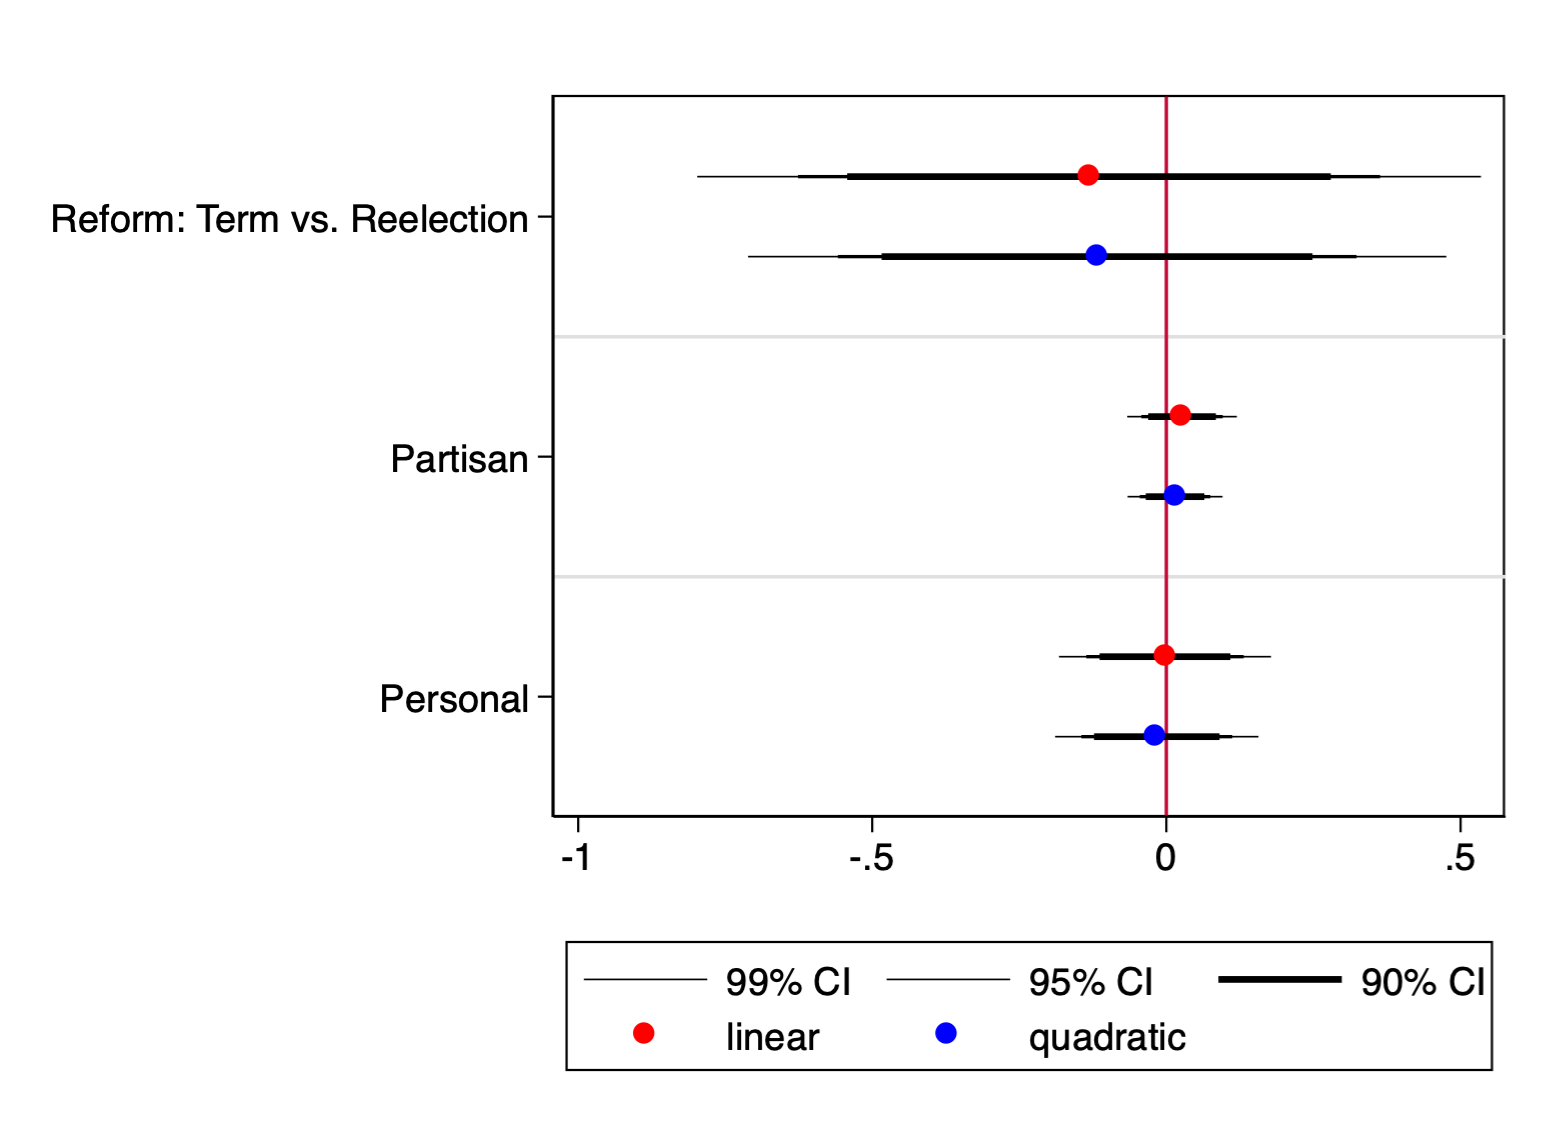
\includegraphics[width=0.9\textwidth]{Chapter2/Figures_incumbency/quality.png}
       \captionsetup{justification=centering}
         
 \textbf{Note:} Figure \ref{fig:quality_trend} shows the average treatment effect of the Term Limit Reform on a dummy indicator of whether candidates hold a professional title. Same optimal bandwidths as those in Table \ref{tab:naive_twfe} are used, as well as the same number of observations.   
     
\end{figure}   

To test for a quality-based incumbency advantage, Figure \ref{fig:quality_trend} shows the difference-in-discontinuity estimator on the indicator of whether a mayor hold a professional title, i.e. the coefficient for the personal incumbency advantage. We observe no difference in the quality of incumbents that barely won the election in $t$ to those that barely lost, before and after the Electoral Reform. In other words, it seems there is no evidence of a quality-based incumbency advantage. However, there could exist a difference in the quality of challengers who out of fear to the experience and ability of incumbents might choose not to run for office, the so called scare-off effect. Sadly, there is no municipal level data on the quality of challengers. To test for potential scare-off effects we would have to compare either a term-limited mayor who was won election once to a term-limited mayor who has won election twice, where both are facing the same election incentives but hold different selection histories. The same could be done by comparing first term mayor that can reelection and has won election once to a mayor that can reelect and has won election twice. This experiment to isolate the election from the selection effect is done by \citet{ashworth_2012}. We leave this test for future research.

Lastly, these estimates do not allow to test for an information-based incumbency advantage. To do so we would need data on whether citizens increased their information reception of incumbents actions and behavior in office. Future work is needed to disentangle the specific information and quality-based mechanisms behind the observed incumbency returns in mayoral elections in Mexico. 

  

\section{Conclusion} 

This paper disentangles the partisan from the personal incumbency advantages. By not disentangling these two components when estimating incumbency electoral returns, most of the literature has failed to correctly identify the valuation citizens have on the electoral system and the existent accountability relationships between parties, politicians and voters. To unbox incumbency advantage into its personal and partisan components, this paper relies on a difference-in-discontinuity of close elections design that exploits the staggered implementation of the 2014 Electoral Reform in Mexico that removed term limits for local mayors. In a setting of close elections, term limit mayors allows us to identify the partisan incumbency returns, while those up for reelection identify both the partisan and personal returns. The difference between these two measures allows for the identification of the personal incumbency advantage. Moreover, the difference-in-difference setup allows us to test for no differential trends of these two type of races prior to the introduction of the reform, while the regression discontinuity of close elections design allows us to reduce the potential of omitted variables, including party, elections and candidates differences. Lastly, we consider only mayors in their first terms which allows us to leave aside selection concerns coming from differences in experience and skills. 

The main result of the paper shows that the implementation of reelection in Mexico led to an incumbency advantage. However, this incumbency advantage can be decomposed into a personal incumbency \emph{advantage} and a partisan incumbency  \emph{disadvantage}. Since the personal incumbency advantage is greater than the partisan incumbency disadvantage, results suggest that reelection makes incumbency a personal affair and may signal a potential party dealignment in Mexican politics. The asymmetric effects also imply parties in Mexico do not hold a credible threat to punish renegade non-term limit mayors any longer. 

The paper further tries to explain the reasons behind the observed incumbency returns. An increase in the revenues and fiscal transfers to municipalities provide strong evidence of a resource-based incumbency advantage. In other words, citizens create a positive incumbency return with candidates who they expect will bring a higher budget or transfer in the future, and not their parties. We also test whether a quality-incumbency advantage exists. While no quality differences are found between term limit and non-term limit incumbents before and after the implementation of the Term Limit Reform, more data is needed to test for potential scare-off effects. It is also important to note that we do not have data on whether citizens increased their information reception of incumbents action, data that could be used to test whether an information-based incumbency advantage explains the observed results.
